\documentclass[a4paper, 12pt]{article}
 
\usepackage[applemac]{inputenc}
\usepackage{graphicx}
\usepackage[french]{babel}
\usepackage[T1]{fontenc}
\usepackage{lmodern}
\usepackage{float}
\usepackage{fullpage}
\usepackage{array}
\usepackage{multirow}
\usepackage[margin = 2cm]{geometry}
\usepackage{amsmath}
 
\begin{document}
 
\title{MLCV Lab 3}
\author{Mathurin \textsc{Massias}}
\date{\today} 
 
\maketitle

\section{Expectation Maximization}

We run K-means 20 times for positive and negative datasets, then pick the initializations giving the lower distortions. For these, we plot distortion as a function of the number of iterations :
\begin{figure}[H]
	\centering
	\noindent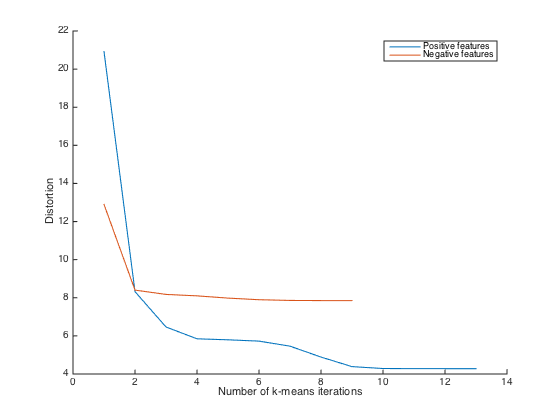
\includegraphics[scale=0.6]{distortion.png}
	\caption{Distortion as a function of number of iterations, for the initializations giving the lower final distortions}
\end{figure}
We confirm that the distortion decreases at each iteration.
\\We also plot the clusters and centroids obtained at convergence:

\begin{figure}[H]
	\centering
	\noindent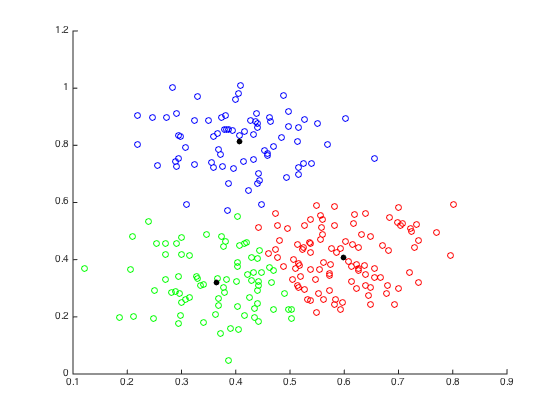
\includegraphics[scale=0.4]{kmeans_pos.png}
	\noindent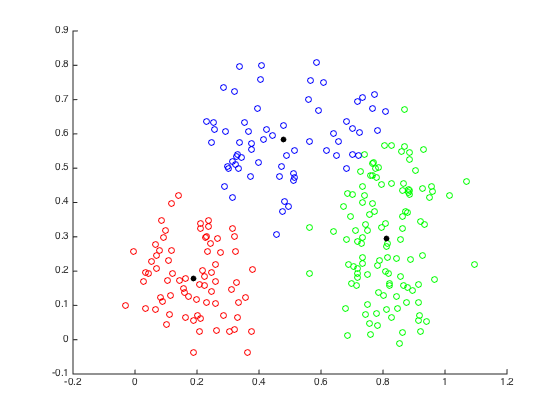
\includegraphics[scale=0.4]{kmeans_neg.png}
	\caption{KMeans results: clusters and centroids (in black). Left : positive features, right : negative features}
\end{figure}
As we can see, the negative clusters are more spread. Since there are 250 points in both positive and negative datasets, it is logical to see that the negative final distortion is higher (be careful, the scales are not the same on the 2 clusters plots). 
%
\\We use these centroids to initialize our EM algorithm (taking as initial covariances, the empirical covariances of the respective datasets).
\begin{figure}[H]
	\centering
	\noindent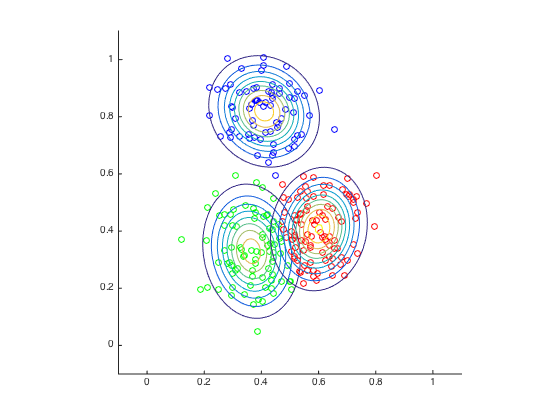
\includegraphics[scale=0.4]{em_pos.png}
	\noindent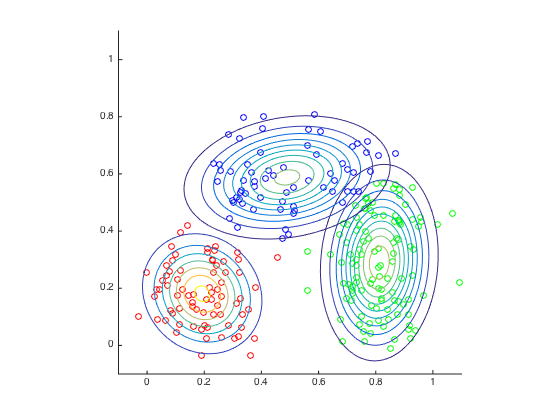
\includegraphics[scale=0.4]{em_neg.png}
	\caption{EM results: clusters and Gaussian densities represented as elliptic level-sets. Left : positive features, right : negative features}
\end{figure}


\begin{figure}[H]
	\centering
	\noindent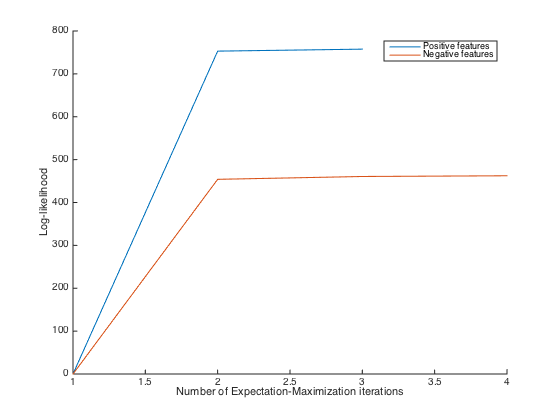
\includegraphics[scale=0.6]{llh.png}
	\caption{Log-likelihood as a function of number of iterations, when initializing with the results of the best Kmeans}
\end{figure}
As we can see, the algorithm converges very quickly, in at most 3 iterations. We confirm that the LLH is increasing at each step.

Since we have the densities for each of the 2 classes, we can compute the posterior probability, and plot its boundaries on top of the dataset :
\begin{figure}[H]
	\centering
	\noindent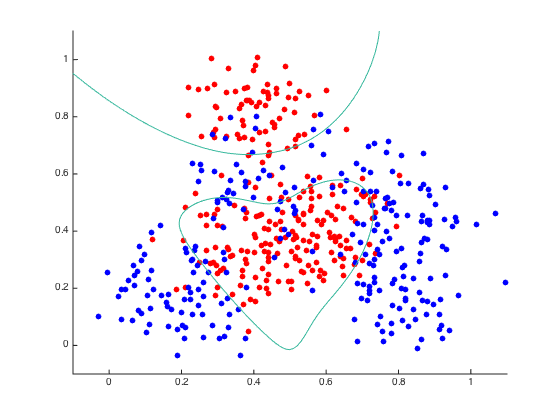
\includegraphics[scale=0.6]{boundaries.png}
	\caption{Original dataset and boundaries found with the posterior probability from EM}
\end{figure}

\section{Sum/Max-Product algorithm}
Forward : message passing 
\\- from 3 and 4 to 2
\\- from 2 and 5 to 1
%
\\ \\Backward : message passing
\\- from 1 to 2 and 5
\\- from 2 to 3 and 4
%
\\[5mm]$Z = \sum\limits_{X_1}{} B(X_1)$, we get $1.9150$.
\\For $P(X_1)$ we get 
$\begin{pmatrix} 0.2914 \\0.5311
    \\0.1775\end{pmatrix} $
    and for $P(X_2)$, $\begin{pmatrix} 0.4543 \\
    0.5457\end{pmatrix} $
    %
%
\\For the given vectors (in the order of the assignment), we found the respective probabilities : 0.0135, 0.0048 and 0.0243.
\\[5mm]If we know $X_5 =1$ etc, this time we get $P(X_3) = \begin{pmatrix}0.1445
    \\0.4913
    \\0.1387
    \\0.2254 \end{pmatrix}, 
   P(X_2) = \begin{pmatrix}
    0.7803
   \\ 0.2197
    \end{pmatrix}$ and $Z =0.0519$


\end{document}